% !TEX encoding = UTF-8
% !TEX TS-program = pdflatex
% !TEX root = ../relazione.tex
% !TEX spellcheck = it-IT
\clearpage
\section{Architettura della soluzione}

L'architettura della soluzione è stata progettata a partire dal codice presente nel repository del ilbro ``Intelligenza Artificiale: Un approccio moderno'', il quale contiene l'implementazione Python dell'algortimo Hill Climbing standard e di alcune classi quali: \texttt{Problem} che definisce l'interfaccia di un problema di ricerca e \texttt{Node} che rappresenta il nodo di un albero di ricerca.

Dal momento che il codice di queste classi si trovava all'interno di un unico modulo Python, è stato necessario apportare opportune modifiche in modo da ottenere un codice più strutturato:

\begin{itemize}
\item Le funzioni di supporto, come la scelta casuale di un massimo, sono state racchiuse nel modulo \texttt{util}:
\item \`{E} stato creato un package \texttt{problem} che contiene la classe astratta \texttt{Problem} e la sua derivata \texttt{NQueens};
\item Le classi relative alla ricerca, ovvero \texttt{Node}, \texttt{HillClimbingSearch} e le altre versioni implementate, sono state racchiuse nel package \texttt{search}.
\end{itemize}

\subsection{problem}

\begin{figure}[ht]
\centering
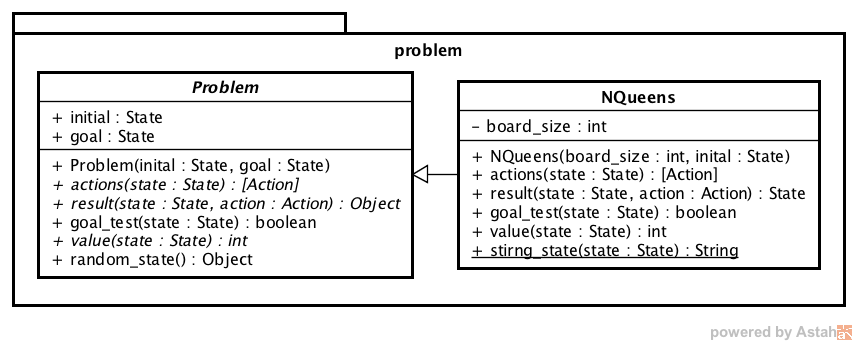
\includegraphics[width=0.8\textwidth]{./immagini/problem_uml.png}
\caption{Diagramma UML del modulo \texttt{problem}.}
\label{fig:uml_problem}
\end{figure}

Per rappresentare un problema di ricerca è stata utilizzata la stessa rappresentazione proposta dal codice del repository e per modellare il problema delle N-Regine è stata creata una nuova classe che deriva da \texttt{Problem}, la quale concretizza i vari metodi astratti.

Gli stati del problema delle N-Regine vengono rappresentati con una lista di interi di lunghezza \textit{N} i cui elementi vanno da \textit{0} a \textit{N-1}. Con questa rappresentazione l'elemento \textit{i-esimo} della lista indica la riga in cui si trova la regina della colonna \textit{i}.

Così facendo non è necessario definire un tipo ad-hoc per la rappresentazione dello stato, è sufficente la lista di interi\footnote{Nei diagrammi UML, quando un metodo riceve come parametro uno stato viene utilizzato il tipo \texttt{State} al posto di \texttt{[int]} per specifcare che si tratta di uno stato, anche se l'implementazione effettiva è una lista di interi}. 

Le azioni del problema vegnono invece rappresentate con una tupla di due interi \texttt{(c,r)} la quale rapppresenta l'azione che sposta la regina della colonna \textit{c} nella riga \textit{r}\footnote{Anche in questo caso, nei diagrammi UML viene utilizzato il tipo \texttt{Action} per indicare la tupla \texttt{(c,r)}}.

\subsection{search}

\begin{figure}[ht]
\centering
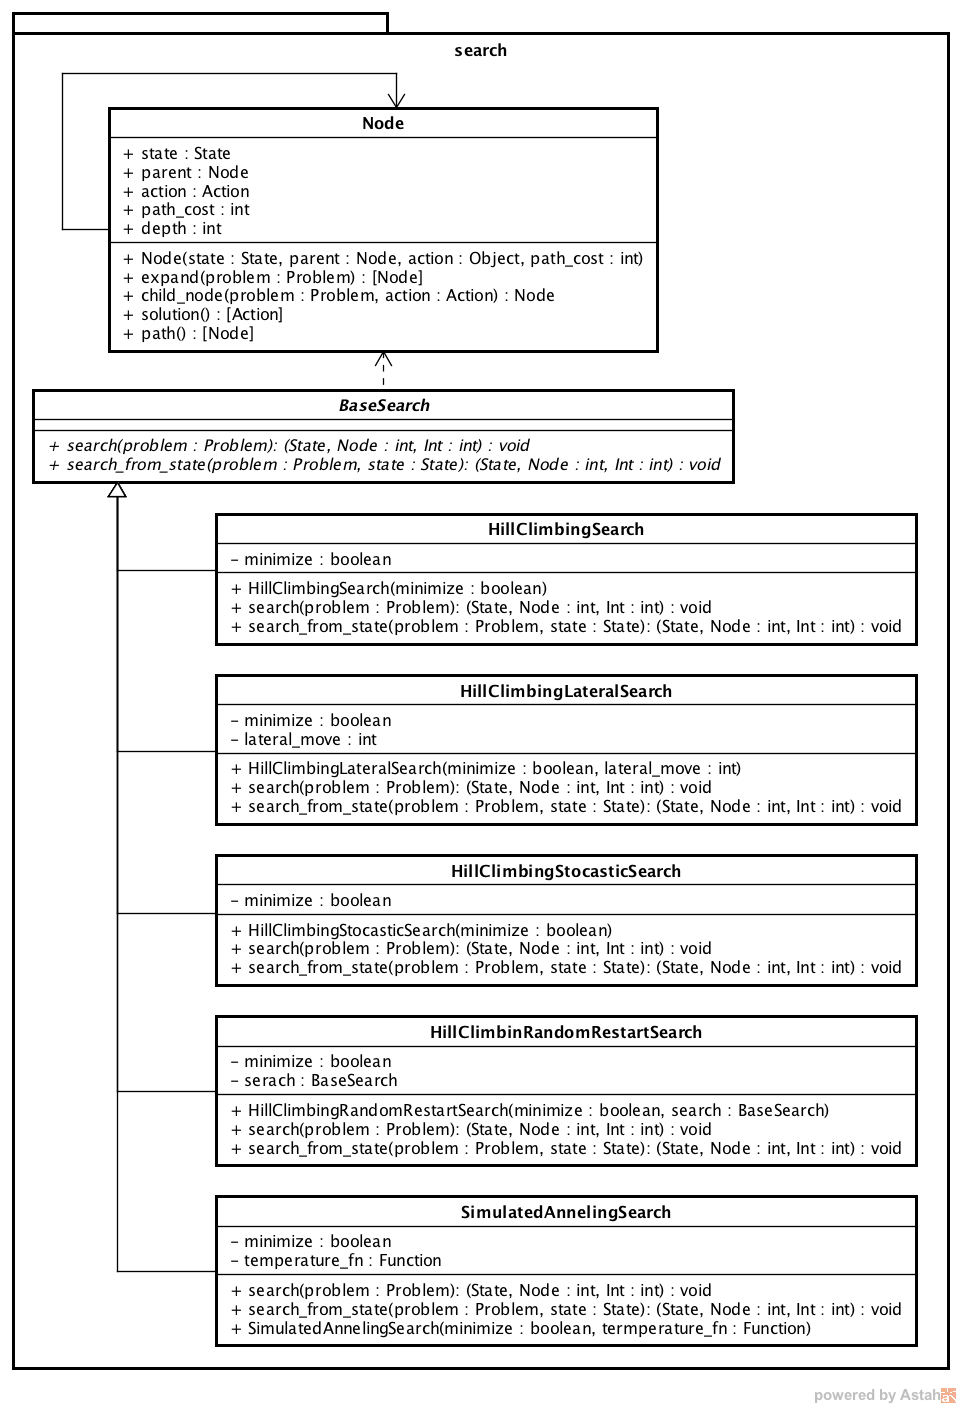
\includegraphics[width=\textwidth]{./immagini/search_uml.png}
\caption{Diagramma uml del modulo \texttt{search}.}
\label{fig:uml_search}
\end{figure}


Tutte le classi che rappresentano un algoritmo di ricerca hanno la stessa classe base \texttt{BaseSearch}, la quale definisce due metodi astratti \texttt{search(problem)} e \texttt{search$\_$from$\_$state(problem, state)}, che permettono rispettivamente di ricerca la soluzione di un problema a partire dallo stato iniziale o da uno stato specifico.

Questi due metodi ritornano una tupla \texttt{(state, node, cnt)} contenente il risultato della ricerca:
\begin{itemize}
\item \texttt{state}: rappresenta lo stato del problema sul quale è terminata la ricerca e non è detto che sia uno stato goal;
\item \texttt{node}: rappresenta il nodo sul quale è terminata la ricerca;
\item \texttt{cnt}: rappresenta il numero di passi che sono stati eseguiti durante la ricerca. Nel caso di una ricerca a riavvio casuale rappresenta il numero di riavvi.
\end{itemize}

Per rappresentare i nodi che vengono visitati dagli algoritmi di ricerca viene utilizzata la classe \texttt{Node}, la quale può essere utilizzata anche per le ricerche ad albero dal momento che contiene informazioni relative al cammino che c'è dal nodo iniziale al nodo corrente e anche il costo di tale cammino.
Anche se queste informazioni non sono necessarie per una ricerca locale sono state mantenute dal momento che rappresentano lo storico dei passaggi fatti dall'algoritmo di ricerca e possono tornare utili per il debug o per visualizzare l'andamento della ricerca.

Le classi che rappresentano gli algoritmi di ricerca sono:
\begin{itemize}
\item \texttt{HillClimbingSearch}: implementa la ricerca Hill Climbing classica. Il costruttore ha come parametro opzionale \texttt{minimize}, un booleano che specifica se la ricerca deve minimizzare o massimizzare il valore della funzione di valutazione.
\item \texttt{HillClimbingStocasticSearch}: implementa la ricerca Hill Climbing stocastica. Anche in questo caso il costruttore ha come parametro \texttt{minimize}.
\item \texttt{HillClimbingLateralSearch}: implementa la ricerca Hill Climbing con mosse laterali. Il costruttore ha due parametri opzionali: \texttt{minimize} e \texttt{lateral$\_$move}.
\item \texttt{HillClimbingRandomRestartSearch}: implementa la ricerca a riavvio casuale. La ricerca da utilizzare può essere specificata con il parametro \texttt{search} del costruttore. Se questo parametro non viene specificato, viene utilizzata la ricerca \texttt{HillClimbingSearch}.
\item \texttt{SimulatedAnnealingSearch}: implementa la ricerca secondo simulated annealing. Il costruttore della classe accetta due parametri, \texttt{minimize} che specifica se il problema di risolvere è di minimizzazione o meno, e \texttt{temperature$\_$fn}, la funzione di raffreddamento. Se non viene specificata una funzione, viene utilizzata la funzione 
\end{itemize}

\begin{align*}
temperature\_fn(t) &= 20 e^{-0,05t} \text{ se }  t < 1000 \\
&= 0  \text{ se }  t \geq 1000
\end{align*}









